\documentclass[conference]{IEEEtran}
\IEEEoverridecommandlockouts

\usepackage[utf8]{inputenc}
\usepackage[T1]{fontenc}
\usepackage[spanish,es-nodecimaldot]{babel}
\usepackage{cite}
\usepackage{amsmath,amssymb,amsfonts}
\usepackage{graphicx}
\usepackage{textcomp}
\usepackage{xcolor}
\usepackage{booktabs}
\usepackage{array}
\usepackage{url}
\usepackage{balance}
\usepackage{tabularx}
\usepackage[hidelinks]{hyperref}
\usepackage{makecell}
\graphicspath{{figuras/}}
\addto\captionsspanish{%
    \renewcommand{\tablename}{Tabla}
    \renewcommand{\figurename}{Figura}
    \renewcommand{\thetable}{\Roman{table}}
}

\def\BibTeX{{\rm B\kern-.05em{\sc i\kern-.025em b}\kern-.08em
    T\kern-.1667em\lower.7ex\hbox{E}\kern-.125emX}}

\def\UrlBreaks{\do\/\do-\do\_}

\begin{document}

\title{GEODETECTOR: un pipeline híbrido basado en inteligencia artificial para la detección, clasificación y geolocalización automatizada de letreros turísticos en rutas y carreteras}

\author{
\IEEEauthorblockN{Felipe Córdova}
\IEEEauthorblockA{\textit{Instituto de Informática} \\
\textit{Universidad Austral de Chile}\\
Valdivia, Chile \\
\texttt{felipe.cordova@alumnos.uach.cl}}
\and
\IEEEauthorblockN{Luis Veas-Castillo}
\IEEEauthorblockA{\textit{Instituto de Informática} \\
\textit{Universidad Austral de Chile}\\
Valdivia, Chile \\
\texttt{luis.veas@uach.cl}}
\and
\IEEEauthorblockN{Christian Lazo}
\IEEEauthorblockA{\textit{Instituto de Informática}\\
\textit{Universidad Austral de Chile}\\
Valdivia, Chile \\
\texttt{christian.lazo@uach.cl}}
}

\maketitle

\begin{abstract}
La información disponible en letreros turísticos instalados en rutas
rurales y carreteras permanece escasamente integrada a sistemas digitales
de inventario territorial. Este artículo presenta GEODETECTOR, un 
pipeline híbrido que combina detección de letreros, sincronización 
GPS, extracción de regiones de interés, reconocimiento óptico de caracteres, 
clasificación semántica por taxonomía turística y visualización de resultados 
georreferenciada. La propuesta fue evaluada con 
videos capturados desde un vehículo en movimiento en tres rutas de la 
Región de Los Lagos, Chile, bajo condiciones reales de iluminación, 
clima y velocidad. El modelo fue entrenado mediante transfer learning 
sobre un dataset propio de 2.000 imágenes etiquetadas de letreros 
capturados principalmente en Chile y Argentina, publicado en IEEE DataPort. La
evaluación experimental consideró cuatro configuraciones de captura, combinando 
dos resoluciones (1080p y 720p) y dos tasas de frames (30 FPS y 15 FPS), 
donde el modelo alcanzó Precisión entre 0,77 y 0,91, Recall 
entre 0,50 y 0,74 y F1-score entre 0,61 y 0,76, mientras que el 
reconocimiento de texto obtuvo un Character Error Rate entre 0,08 y 0,27. La
evaluación end-to-end mostró que el pipeline completó 
automáticamente la detección, lectura, clasificación y 
georreferenciación del 57,1\% de los letreros turísticos correctamente 
detectados en la configuración original de captura. Los resultados 
evidencian la viabilidad de utilizar visión artificial para apoyar el 
inventario de infraestructura turística vial en entornos no controlados.
\end{abstract}

\begin{IEEEkeywords}
visión artificial, YOLO, transfer learning, OCR, georreferenciación, letreros turísticos, inteligencia artificial, rutas rurales.
\end{IEEEkeywords}

\section{Introducción}

Las rutas y carreteras rurales concentran una cantidad relevante de 
información territorial que no siempre se encuentra disponible en 
plataformas digitales. En particular, muchos emprendimientos turísticos,
servicios de alimentación, alojamientos y actividades recreativas se 
anuncian mediante letreros instalados al borde del camino. Estos elementos
cumplen una función informativa para los viajeros, pero también 
constituyen una fuente de datos potencialmente valiosa para municipios, 
organismos de turismo y planificadores territoriales. Sin embargo, su 
registro suele depender de levantamientos manuales, costosos y 
difíciles de actualizar.

Los avances recientes en detección de objetos y reconocimiento de texto 
en escenas naturales permiten abordar este problema desde una perspectiva 
automatizada. Modelos de detección como YOLO han demostrado alta 
eficiencia en escenarios viales y aplicaciones de transporte 
inteligente \cite{letreros-transito-pare-semaforo-1,yolo-vehiculos}. Asimismo, 
los sistemas de reconocimiento óptico de caracteres (OCR) y Scene Text 
Recognition (STR) han ampliado la capacidad de extraer texto desde 
imágenes complejas \cite{soni2025performance,ocr-curvo}. No obstante, 
la señalética turística rural presenta dificultades particulares: 
variabilidad visual, tipografías no estandarizadas, materiales 
artesanales, deterioro físico, bajo contraste, vegetación que obstruye 
parcialmente los letreros, condiciones climáticas variables, y 
condiciones externas al objeto de interés como la velocidad del 
vehículo, la presencia de suciedad en el parabrisas o las limitaciones 
propias de la cámara de un smartphone durante la captura.

La literatura sobre señales de tránsito se concentra principalmente 
en señalética regulada, con colores, formas y diseños normalizados
\cite{TT100K-Dataset,gtsdb-dataset}. En cambio, los letreros turísticos 
rurales y comerciales no estandarizados han sido escasamente estudiados, 
especialmente en contextos latinoamericanos. Además, la detección 
visual por sí sola no entrega la posición geográfica real del objeto,
por lo que es necesario sincronizar el video con datos de geolocalización
 \cite{roboflow-georeferencing}. Esta integración entre visión 
artificial, OCR, clasificación semántica y georreferenciación 
constituye el foco de este trabajo.

Este artículo presenta GEODETECTOR, un pipeline híbrido orientado a 
detectar, interpretar y geolocalizar letreros turísticos capturados 
desde vehículos en movimiento. La propuesta se valida mediante videos 
reales adquiridos en rutas de la Región de Los Lagos, Chile, considerando
distintas resoluciones, tasas de frames por segundo y condiciones 
climáticas. Las principales contribuciones son: \textbf{(i)} la 
construcción de un dataset propio de 2.000 imágenes etiquetadas de 
letreros rurales, urbanos y turísticos, publicado en IEEE DataPort; 
\textbf{(ii)} el diseño de un pipeline end-to-end que integra detección, 
OCR, clasificación semántica y geolocalización; y \textbf{(iii)} la evaluación 
experimental en condiciones reales, incluyendo una medición integral 
que muestra que el pipeline logra completar automáticamente el flujo 
para el 57,1\% de los letreros turísticos correctamente detectados.

\section{Trabajos relacionados}

La detección de objetos en video ha evolucionado de manera significativa 
gracias a modelos profundos de una y dos etapas. Faster R-CNN prioriza
precisión mediante propuestas de región \cite{rnn-faster}, mientras que 
la familia YOLO privilegia velocidad de inferencia y ha sido ampliamente 
adoptada en aplicaciones vehiculares \cite{comparacion-yolo-rnn,yolo-vehiculos}. 
Sin embargo, distintos trabajos han reportado degradación de desempeño 
ante lluvia, niebla, baja iluminación y ruido visual 
\cite{yolo-escenarios-naturales}. Estos factores son especialmente 
relevantes cuando los objetos aparecen durante pocos segundos y a 
distancias variables.

En reconocimiento de texto, el OCR tradicional ha sido utilizado en 
dominios como banca, compras en línea y salud \cite{ocr-banco,ocr-compras-en-linea,ocr-salud}. 
En escenas naturales, el problema es más complejo debido a fondos no 
uniformes, perspectivas, rotaciones, tipografías diversas y oclusiones. 
Los enfoques STR han mejorado la lectura de texto irregular, pero muchos 
benchmarks se concentran en señalética urbana o texto en inglés, sin 
representar adecuadamente letreros artesanales de rutas rurales 
latinoamericanas \cite{icdar,ocr-curvo}.

Los datasets de señales de tránsito, como TT-100K (Tsinghua-Tencent 100K) y
GTSDB (German Traffic Sign Detection Benchmark), han permitido 
avances importantes en detección de señalética regulada 
\cite{TT100K-Dataset,gtsdb-dataset}. No obstante, sus clases y 
distribuciones visuales difieren del dominio turístico rural, donde 
predominan letreros informales, materiales heterogéneos y ausencia de 
estándares gráficos. Esta diferencia produce un problema de cambio de 
dominio o \textit{domain shift}, frente al cual el transfer learning es 
una alternativa efectiva cuando se dispone de datos específicos limitados 
\cite{domain-shift,transfer-learning,transfer-learning-yolo}. GEODETECTOR 
aborda esta brecha mediante un dataset propio y un pipeline integrado que 
combina visión, texto y geolocalización.

\section{Metodología}

\subsection{Visión general del pipeline}

GEODETECTOR se organiza en dos etapas, como se muestra en la 
Figura~\ref{fig:pipeline}. La \textbf{Etapa 1} construye el modelo de detección
mediante un dataset etiquetado, su división en entrenamiento, validación y
prueba, y el fine-tuning de un modelo YOLO11m. La \textbf{Etapa 2} implementa 
el modelo en un escenario de captura vehicular: se procesa el video, se
sincroniza con la traza GPS, se extraen regiones de interés (ROI), se 
aplica OCR, se clasifica semánticamente el contenido textual y se 
visualizan los resultados en un mapa.

\begin{figure*}[t]
\centering
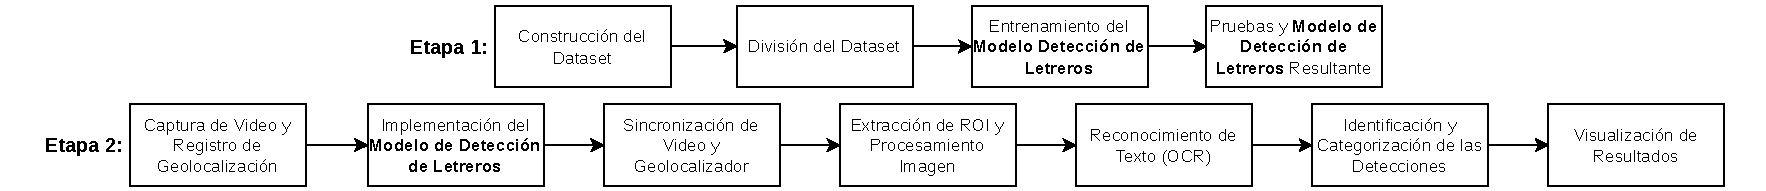
\includegraphics[width=0.94\textwidth]{figura2.pdf}
\caption{Pipeline general de GEODETECTOR. La Etapa 1 construye y valida el modelo de detección; la Etapa 2 integra captura, sincronización GPS, OCR, clasificación semántica y visualización georreferenciada.}
\label{fig:pipeline}
\end{figure*}

\subsection{Construcción del dataset}

El dataset fue construido a partir de recorridos realizados entre enero y 
septiembre de 2025 en cinco regiones de Chile y una localidad de Argentina.
Las imágenes fueron capturadas con un smartphone Samsung Galaxy S23 en 
contextos urbanos, rurales y turísticos, considerando variabilidad de 
distancia, ángulo, iluminación, materialidad y estado de conservación de 
los letreros. Cada imagen fue etiquetada manualmente mediante Label 
Studio \cite{labelstudio2026}, encerrando cada letrero visible 
con un bounding box que delimita su área exacta, usando una clase única: \textit{signboard} (letrero). 
Las etiquetas fueron exportadas en formato TXT estándar de YOLO, 
donde cada archivo contiene una línea por letrero presente en la 
imagen, con el formato \texttt{class x\_center y\_center width height}, 
siendo todos los valores normalizados entre 0 y 1 respecto a las 
dimensiones de la imagen, y la 
metadata se consolidó mediante scripts en Python \cite{python2026}. Para 
resguardar privacidad, se difuminaron rostros, patentes de vehículos, códigos QR y 
números telefónicos visibles mediante GIMP \cite{gimp2026}. El dataset está 
publicado en IEEE DataPort \cite{ieee-dataset}. La Tabla~\ref{tab:dataset} resume la distribución 
geográfica del dataset, incluyendo las regiones, las 
localidades principales y la cantidad de imágenes 
recolectadas por zona.

\begin{table}[!t]
\caption{Distribución geográfica de las imágenes recolectadas.}
\label{tab:dataset}
\centering
\footnotesize
\begin{tabular}{p{1.8cm}p{4.1cm}r}
\toprule
Región & Localidades principales & Cantidad \\
\midrule
La Araucanía & Pucón, Villarrica, Caburgua, Licanray, Loncoche & 979 \\
Los Lagos & Puerto Montt, Frutillar, Calbuco, Puerto Varas & 542 \\
Los Ríos & Valdivia, Panguipulli, Lago Ranco, Lanco & 467 \\
O'Higgins & Quinta de Tilcoco, Rancagua & 7 \\
El Maule & Colbún, San Clemente & 2 \\
Argentina & San Carlos de Bariloche & 3 \\
\bottomrule
\end{tabular}
\end{table}

\subsection{Modelo de detección}

Se utilizó YOLO11m como modelo base, seleccionando la variante 
\textit{medium} por su equilibrio entre capacidad de representación y 
generalización para el tamaño del dataset. Se aplicó transfer learning a partir de pesos preentrenados y 
fine-tuning sobre el dataset propio. Las imágenes de entrada fueron 
configuradas a 640$\times$640 píxeles, tamaño al que YOLO redimensiona 
internamente mediante \textit{letterboxing} \cite{letterbox-yolo}, 
preservando la relación de aspecto de las imágenes originales del 
dataset que presentan dimensiones superiores \cite{yolo11_ultralytics}. 
El entrenamiento se realizó con 50 épocas y parada temprana con 
paciencia de 5 épocas. La división de datos fue 70\% entrenamiento, 
15\% validación y 15\% prueba, resultando en 1.400, 300 y 300 imágenes
respectivamente. La Tabla~\ref{tab:train_metrics} resume el 
desempeño final del detector en validación, evitando incluir curvas de 
entrenamiento para ajustarse al límite de extensión del artículo.

\begin{table}[!t]
\caption{Métricas resumidas del modelo YOLO11m personalizado.}
\label{tab:train_metrics}
\centering
\begin{tabular}{lc}
\toprule
Métrica & Valor \\
\midrule
Precisión & 0,88 \\
Recall & 0,83 \\
mAP@50 & 0,92 \\
mAP@50:95 & 0,74 \\
\bottomrule
\end{tabular}
\end{table}

La Figura~\ref{fig:detecciones} muestra ejemplos de detecciones obtenidas 
sobre imágenes del conjunto de prueba. Estas detecciones permiten observar
la respuesta del modelo ante diversidad de formas, materiales, distancias 
y condiciones de iluminación.

\begin{figure}[!t]
\centering
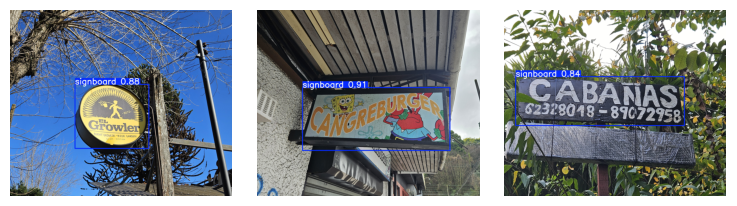
\includegraphics[width=0.98\columnwidth]{figura5.pdf}
\caption{Ejemplos de detecciones realizadas por el modelo YOLO11m personalizado sobre letreros con distinta apariencia visual.}
\label{fig:detecciones}
\end{figure}

\subsection{OCR, taxonomía y geolocalización}

Cada detección con confianza superior a 0,5 se recorta como ROI y se 
procesa mediante transformación a escala de grises y thresholding, técnica
utilizada para mejorar el contraste previo al OCR 
\cite{thresholding-para-mejorar-ocr}. El reconocimiento de texto se 
realiza con PaddleOCR \cite{paddleocr,paddleocr2}, reteniendo resultados 
con confianza superior a 0,5. Luego, el texto se normaliza y se compara 
contra una taxonomía de palabras clave basada en servicios turísticos 
definidos por el Servicio Nacional del Turismo de Chile 
\cite{taxonomia-gobierno}, complementada con términos identificados 
durante la recolección de datos en terreno. La comparación usa 
coincidencia exacta y similitud difusa para tolerar errores de 
OCR \cite{fuzzy-matching}. La Tabla~\ref{tab:taxonomia} resume la taxonomía
utilizada.

\begin{table}[!t]
\caption{Taxonomía de clasificación semántica de letreros turísticos.}
\label{tab:taxonomia}
\centering
\footnotesize
\begin{tabular}{p{1.7cm}cp{4.1cm}}
\toprule
Categoría & Palabras clave & Ejemplos \\
\midrule
Alojamiento & 17 & cabaña, hostal, hotel, hospedaje, apart hotel \\
Alimentación & 73 & restaurant, picada, almuerzos, minimarket, comida casera \\
Recreativa & 56 & rafting, cabalgatas, trekking, playa, artesanías \\
Otros & -- & venta de terrenos, talleres, tránsito u otra señalética no turística \\
\bottomrule
\end{tabular}
\end{table}

La geolocalización se obtiene sincronizando temporalmente el video con una
traza GPX registrada mediante GeoTracker \cite{geotracker}. Se extrae la 
hora de finalización y duración del video con pymediainfo
\cite{pymediainfo}; luego se calcula la hora de inicio 
como $t_{inicio}=t_{fin}-D$, donde $D$ es la duración en segundos. La 
traza GPS se filtra a un punto por segundo para asociar cada frame 
procesado con su coordenada geográfica. Los resultados se consolidan con 
Pandas \cite{pandas} y se visualizan en un sistema de información geográfica (SIG).

\section{Configuración experimental}

El pipeline fue ejecutado en el supercomputador Patagón de la Universidad 
Austral de Chile \cite{patagon}. Para entrenamiento, inferencia y OCR se 
utilizaron recursos GPU, principalmente NVIDIA L40, mientras que tareas de 
sincronización y consolidación fueron ejecutadas con menor demanda 
computacional. El desarrollo se realizó en Python, empleando Ultralytics, 
PaddleOCR, OpenCV \cite{opencv}, Pandas y herramientas auxiliares como 
FFmpeg para generar variantes de resolución y FPS \cite{ffmpeg}.

La evaluación utilizó tres videos reales capturados desde un vehículo a 
velocidades entre 50 y 70 km/h. Cada video original fue grabado en 1080p 
a 30 FPS y transformado en tres variantes: 1080p a 15 FPS, 720p a 30 FPS y 
720p a 15 FPS. En total, se evaluaron 12 escenarios. La 
Tabla~\ref{tab:escenarios} resume las condiciones de captura. LR 
corresponde al total de letreros reales observados y LRT a los letreros 
reales turísticos según la taxonomía.

\begin{table*}[!t]
\caption{Escenarios experimentales evaluados.}
\label{tab:escenarios}
\centering
\footnotesize
\begin{tabular}{llcccccccc}
\toprule
Video & Sector & Hora & Duración & Periodo & Clima & Velocidad & LR & LRT & Configuraciones \\
\midrule
V1 & Carretera Austral & 11:13 & 4:03 min & Mañana & Lluvia & 50--70 km/h & 87 & 23 & 1080p/720p; 30/15 FPS \\
V2 & Río Maullín & 10:17 & 4:13 min & Mañana & Neblina & 50--70 km/h & 34 & 4 & 1080p/720p; 30/15 FPS \\
V3 & Camino a Ensenada & 16:52 & 5:58 min & Tarde & Despejado & 50--70 km/h & 91 & 19 & 1080p/720p; 30/15 FPS \\
\bottomrule
\end{tabular}
\end{table*}

Para detección se calcularon Precisión, Recall y F1-score a partir de 
verdaderos positivos (TP), falsos positivos (FP) y falsos negativos (FN), 
usando un conteo manual frame a frame como ground truth 
\cite{ibm_ground_truth}. Para OCR se utilizó Character Error Rate (CER), 
calculado con distancia de edición de Levenshtein 
\cite{levenshtein1966binary,transkribus-cer}.

\section{Resultados}

\subsection{Detección y OCR}

La Tabla~\ref{tab:resumen_resultados} resume el desempeño por video y 
configuración. La Precisión se mantiene relativamente estable entre 0,77 y
0,91, lo que indica que el modelo controla razonablemente los falsos 
positivos en condiciones reales. El Recall presenta mayor variabilidad, 
entre 0,50 y 0,74, reflejando la dificultad de detectar letreros que 
aparecen brevemente en escena o bajo degradación visual. El F1-score 
fluctúa entre 0,61 y 0,76. En OCR, los valores de CER varían entre 0,08 
y 0,27, con mejores resultados en 1080p a 30 FPS.

\begin{table*}[!t]
\caption{Resumen de resultados de detección y OCR por configuración.}
\label{tab:resumen_resultados}
\centering
\footnotesize
\begin{tabular}{cccccccc}
\toprule
Video & Resolución & FPS & Precisión & Recall & F1-score & CER prom. & Interpretación OCR \\
\midrule
V1 & 1080p & 30 & 0,87 & 0,63 & 0,73 & 0,13 & Aceptable \\
V1 & 1080p & 15 & 0,85 & 0,60 & 0,70 & 0,23 & Deficiente \\
V1 & 720p & 30 & 0,91 & 0,60 & 0,72 & 0,16 & Aceptable \\
V1 & 720p & 15 & 0,88 & 0,52 & 0,65 & 0,22 & Deficiente \\
V2 & 1080p & 30 & 0,84 & 0,62 & 0,71 & 0,08 & Bueno \\
V2 & 1080p & 15 & 0,78 & 0,74 & 0,76 & 0,27 & Deficiente \\
V2 & 720p & 30 & 0,86 & 0,53 & 0,66 & 0,16 & Aceptable \\
V2 & 720p & 15 & 0,77 & 0,50 & 0,61 & 0,16 & Aceptable \\
V3 & 1080p & 30 & 0,85 & 0,63 & 0,72 & 0,10 & Bueno \\
V3 & 1080p & 15 & 0,81 & 0,67 & 0,73 & 0,20 & Aceptable \\
V3 & 720p & 30 & 0,82 & 0,55 & 0,66 & 0,24 & Deficiente \\
V3 & 720p & 15 & 0,89 & 0,59 & 0,72 & 0,21 & Deficiente \\
\bottomrule
\end{tabular}
\end{table*}

En términos generales, la reducción a 15 FPS afecta tanto la detección 
como el OCR, especialmente cuando los letreros aparecen durante pocos 
frames o cuando existen lluvia, neblina o desenfoque por movimiento. La 
resolución también influye, aunque el efecto observado en OCR sugiere que 
la disponibilidad temporal de frames nítidos es tan importante como la 
cantidad de píxeles. La configuración 1080p a 30 FPS presenta el mejor 
equilibrio general, con valores de OCR buenos o aceptables en los tres 
videos.

\subsection{Evaluación end-to-end}

La evaluación integral considera el flujo completo que recibe el usuario: 
detección del letrero, extracción de texto, clasificación semántica, 
evaluación de calidad informativa y georreferenciación. En la configuración
original 1080p a 30 FPS, V1 contenía 23 letreros turísticos reales, de los
cuales 21 fueron correctamente detectados; 11 superaron el filtro de 
confianza OCR y fueron evaluados y clasificados. En V2, 3 de 4 letreros 
turísticos fueron detectados y los 3 pasaron el filtro OCR. En V3, 18 de 19
letreros turísticos fueron detectados, pero solo 10 superaron el umbral OCR.

En conjunto, el pipeline logró evaluar y clasificar exitosamente 24 de 42 
letreros turísticos correctamente detectados, lo que corresponde a una 
tasa end-to-end de 57,1\%. Este resultado muestra que la etapa de OCR 
actúa como el principal filtro del pipeline. Aunque el detector identifica 
la mayor parte de los letreros turísticos visibles, cerca de la mitad de 
ellos puede perderse antes de la clasificación final debido a baja nitidez,
deterioro, ángulo de captura, reflejos o desenfoque por movimiento.

La Figura~\ref{fig:endtoend} ilustra un caso exitoso de procesamiento 
completo: se captura el video y la traza GPS, el modelo detecta el 
letrero, se sincronizan ambas fuentes, se extrae la ROI y se procesa, el OCR recupera texto 
con alta confianza, la taxonomía asigna una categoría turística y el resultado
se visualiza sobre un mapa con coordenadas asociadas.

\begin{figure*}[t]
\centering
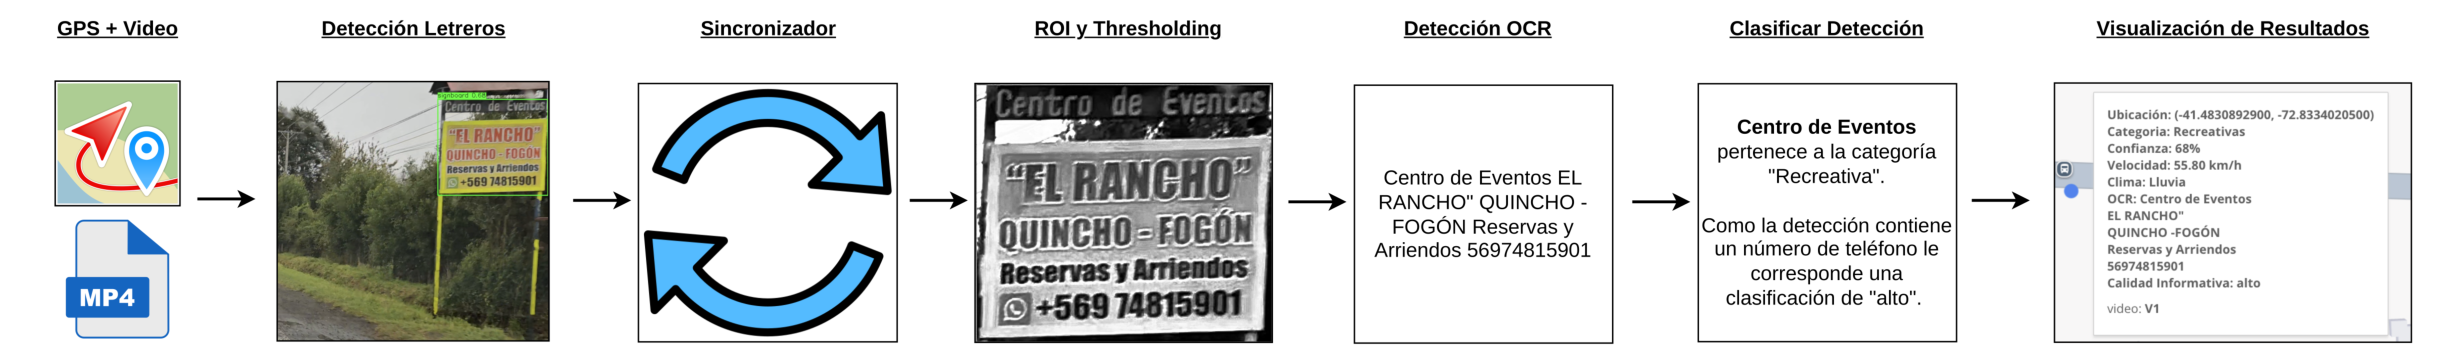
\includegraphics[width=0.94\textwidth]{figura7.pdf}
\caption{Ejemplo de ejecución end-to-end de GEODETECTOR sobre un letrero turístico capturado en ruta.}
\label{fig:endtoend}
\end{figure*}

\subsection{Visualización georreferenciada}

Los resultados consolidados fueron representados en un SIG. 
La Figura~\ref{fig:mapa} muestra la distribución geográfica de las 
detecciones obtenidas en los tres videos. Cada punto representa un letrero 
detectado y georreferenciado; al seleccionarlo, el usuario puede revisar 
coordenadas, categoría, texto reconocido, confianza de detección, 
condiciones de captura y calidad informativa. Este componente permite 
transformar detecciones individuales en una herramienta de apoyo para 
inventarios territoriales.

\begin{figure}[!t]
\centering
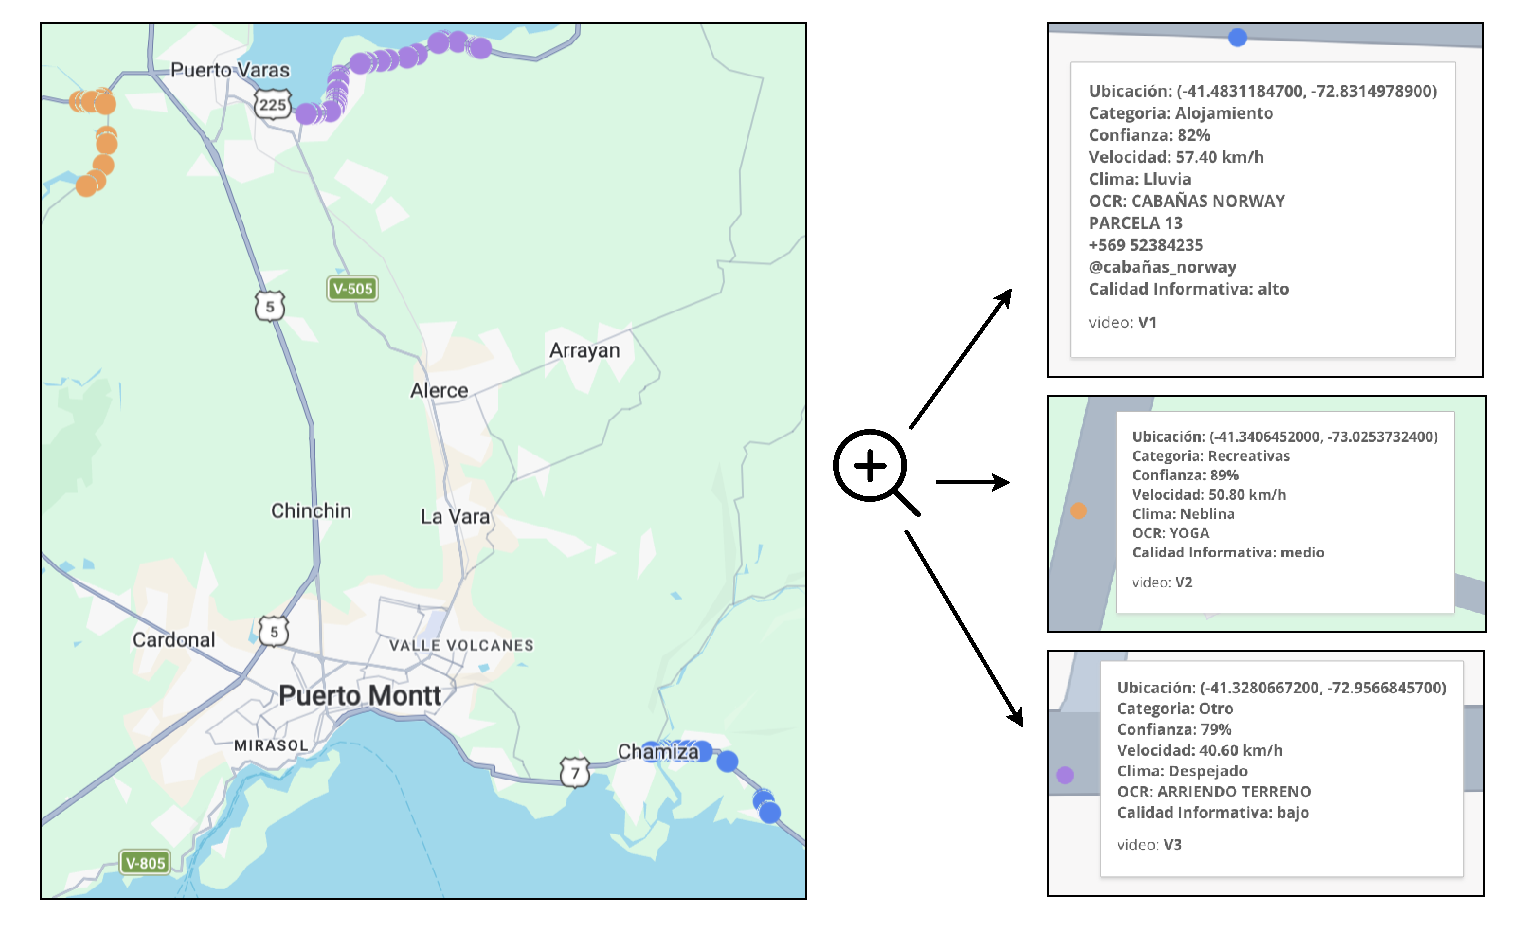
\includegraphics[width=0.98\columnwidth]{figura8.pdf}
\caption{Mapa interactivo con la distribución geográfica de las detecciones obtenidas en los tres videos de prueba.}
\label{fig:mapa}
\end{figure}

\section{Discusión}

Los resultados evidencian que GEODETECTOR es viable para detectar y 
geolocalizar letreros turísticos en condiciones reales de captura vehicular. 
La Precisión promedio obtenida en video se mantiene cercana al desempeño de
validación del detector, lo que respalda la decisión de entrenar un modelo
especializado en lugar de depender de clases generales de YOLO. Esta 
observación es consistente con trabajos que muestran degradación por 
cambio de dominio cuando el dataset de entrenamiento no representa el 
escenario de aplicación \cite{domain-shift,dataset-no-existentes}.

La caída en Recall respecto al obtenido durante el entrenamiento era esperable, ya 
que la evaluación en video introduce factores ausentes en imágenes 
estáticas: movimiento del vehículo, tiempo limitado de aparición del 
letrero, vibración de cámara, lluvia, neblina y oclusión parcial. Estos 
efectos han sido reportados previamente en análisis de robustez de 
detectores bajo condiciones climáticas realistas 
\cite{yolo-escenarios-naturales}. En este sentido, el aporte del trabajo no
está en obtener una detección perfecta, sino en cuantificar de manera 
transparente el desempeño de un pipeline completo bajo condiciones no 
controladas.

El módulo OCR constituye el principal cuello de botella. Aunque PaddleOCR 
permite leer texto en múltiples idiomas y escenas complejas, su desempeño 
depende fuertemente de la calidad de la ROI recibida. La tasa end-to-end 
de 57,1\% muestra que detectar el letrero no basta: también se requiere 
disponer de frames suficientemente nítidos para extraer texto útil. Las 
configuraciones de 1080p a 30 FPS ofrecen mejores condiciones para 
recuperar texto, mientras que 15 FPS reduce la probabilidad de seleccionar
un frame legible.

La Figura~\ref{fig:limitaciones} muestra ejemplos de limitaciones observadas.
Algunos falsos positivos se producen por objetos rectangulares o planos, 
como laterales de camiones, banderas ondeando o estructuras viales. También se 
detectan señales de tránsito convencionales que comparten rasgos visuales 
con letreros, pero que no pertenecen al dominio turístico. Estos casos 
sugieren que futuras versiones podrían incorporar una segunda etapa de 
filtrado visual, modelos multimodales o clasificadores específicos para 
distinguir señalética turística de otros objetos viales.

\begin{figure}[!t]
\centering
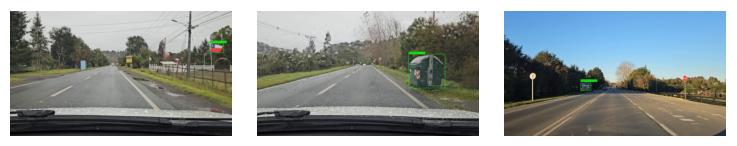
\includegraphics[width=0.98\columnwidth]{figura9.pdf}
\caption{Ejemplos de limitaciones: falsos positivos y detecciones sobre objetos visualmente similares a letreros.}
\label{fig:limitaciones}
\end{figure}

\section{Conclusiones}

Este artículo presentó GEODETECTOR, un pipeline híbrido para detección, 
reconocimiento de texto, clasificación semántica y georreferenciación de 
letreros turísticos capturados desde vehículos en movimiento. La propuesta
integra un detector YOLO11m entrenado con un dataset propio de 2.000 
imágenes, procesamiento de ROI, OCR, una taxonomía turística basada en 
palabras clave y sincronización GPS para visualización en mapa.

Los experimentos realizados sobre tres rutas reales de la Región de Los 
Lagos, evaluados en cuatro configuraciones combinando resoluciones de 
720p y 1080p con tasas de captura de 15 FPS y 30 FPS, muestran que el 
detector alcanza Precisión entre 0,77 y 0,91, Recall entre 0,50 y 0,74 
y F1-score entre 0,61 y 0,76. El OCR obtuvo valores de CER entre 0,08 
y 0,27, confirmando que la lectura de texto en movimiento es la etapa 
más sensible del pipeline. En evaluación end-to-end, el sistema completó 
automáticamente el flujo para el 57,1\% de los letreros turísticos 
correctamente detectados.

Como trabajo futuro se proyecta ampliar el dataset con nuevas regiones, 
evaluar técnicas de super-resolución \cite{ultralytics_super_resolution} y corrección de desenfoque \cite{correcion-desenfoque}, 
desarrollar una aplicación móvil que capture video y GPS de manera 
integrada, y migrar el almacenamiento de resultados hacia una base de 
datos geoespacial. También resulta relevante explorar procesamiento en el 
borde para aproximar el pipeline a una ejecución en tiempo real desde el 
vehículo.

\section*{Agradecimientos}

Esta investigación fue apoyada por el supercomputador Patagón de la 
Universidad Austral de Chile (FONDEQUIP EQM180042).

\balance
\bibliographystyle{IEEEtran}
\bibliography{sample}

\end{document}
